\documentclass[border=3pt]{standalone}
\usepackage{tikz}
\usetikzlibrary{arrows.meta,calc,positioning}
\tikzset{pin/.style={-{Stealth[length=5pt]}},
  fa/.style={draw, thick, minimum width=15mm, minimum height=15mm, font=\sffamily\small}}
\begin{document}
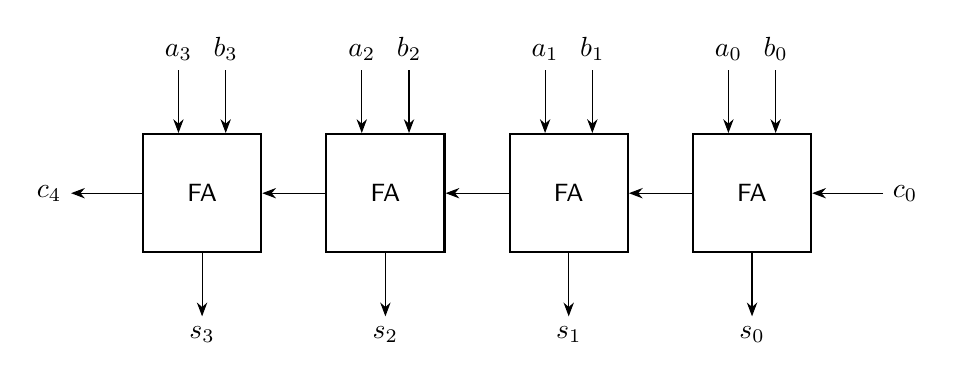
\begin{tikzpicture}[font=\sffamily, node distance=8mm]
  \node[fa] (f0) {FA};
  \node[fa, left=of f0] (f1) {FA};
  \node[fa, left=of f1] (f2) {FA};
  \node[fa, left=of f2] (f3) {FA};
  \foreach \n/\i in {f0/0,f1/1,f2/2,f3/3}{
    % a,b inputs on top
    \draw[pin] ($(\n.north)+(-3mm,8mm)$) node[above]{$a_\i$} -- ($(\n.north)+(-3mm,0)$);
    \draw[pin] ($(\n.north)+(3mm,8mm)$) node[above]{$b_\i$} -- ($(\n.north)+(3mm,0)$);
    % sum on bottom
    \draw[pin] (\n.south) -- ++(0,-8mm) node[below]{$s_\i$};}
  % carry chain (right to left)
  \draw[pin] ($(f0.east)+(9mm,0)$) node[right]{$c_0$} -- (f0.east);
  \draw[pin] (f0.west) -- (f1.east);
  \draw[pin] (f1.west) -- (f2.east);
  \draw[pin] (f2.west) -- (f3.east);
  \draw[pin] (f3.west) -- ++(-9mm,0) node[left]{$c_4$};
\end{tikzpicture}
\end{document}
